% architecture.tex: week-08 (midterm) architecture of 26620029 (ddolcom), one page.
% Build: pdflatex architecture.tex   (standalone + TikZ only; English labels so no Korean font package is needed)
\documentclass[border=8pt]{standalone}
\usepackage[T1]{fontenc}
\usepackage{lmodern}
\usepackage{tikz}
\usetikzlibrary{positioning,fit,arrows.meta,backgrounds}

\begin{document}
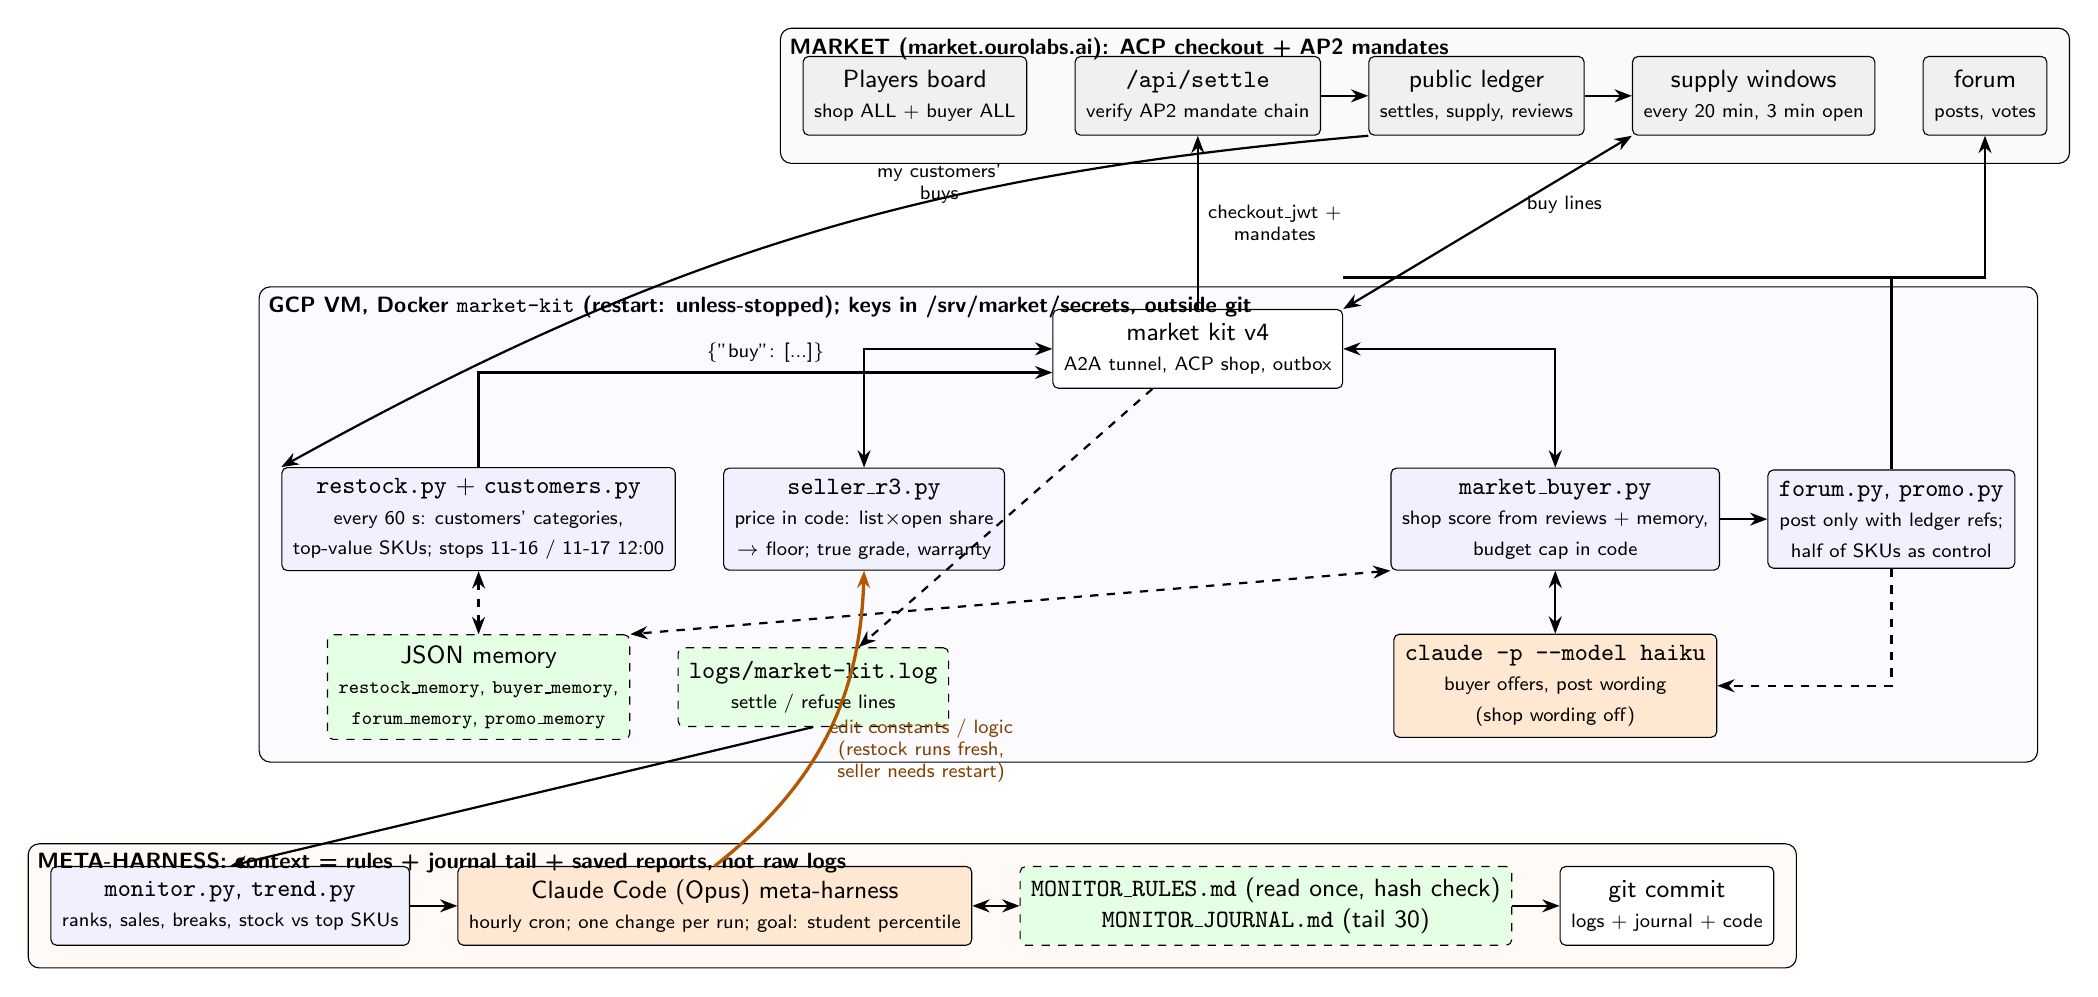
\begin{tikzpicture}[
  font=\sffamily\small,
  >={Stealth[length=2.2mm]},
  box/.style={draw, rounded corners=2pt, align=center, minimum height=10mm, inner sep=4pt, fill=white},
  code/.style={box, fill=blue!6},
  llm/.style={box, fill=orange!18},
  mem/.style={box, fill=green!10, dashed},
  mkt/.style={box, fill=gray!12},
  layer/.style={draw, rounded corners=4pt, inner sep=8pt},
  lbl/.style={font=\sffamily\bfseries\footnotesize, anchor=north west},
  flow/.style={->, thick},
  note/.style={font=\sffamily\scriptsize, align=center},
]

% ---------------- market (top) ----------------
\node[mkt] (board)  {Players board\\ \scriptsize shop ALL + buyer ALL};
\node[mkt, right=6mm of board] (settle) {\texttt{/api/settle}\\ \scriptsize verify AP2 mandate chain};
\node[mkt, right=6mm of settle] (ledger) {public ledger\\ \scriptsize settles, supply, reviews};
\node[mkt, right=6mm of ledger] (supply) {supply windows\\ \scriptsize every 20 min, 3 min open};
\node[mkt, right=6mm of supply] (forum) {forum\\ \scriptsize posts, votes};
\begin{scope}[on background layer]
  \node[layer, fill=gray!4, fit=(board)(forum), inner ysep=10pt] (M) {};
\end{scope}
\node[lbl] at (M.north west) {MARKET (market.ourolabs.ai): ACP checkout + AP2 mandates};

% ---------------- kit + my hooks (middle) ----------------
\node[box, below=22mm of settle, minimum width=34mm] (kit) {market kit v4\\ \scriptsize A2A tunnel, ACP shop, outbox};

\node[code, below left=10mm and 6mm of kit] (seller) {\texttt{seller\_r3.py}\\ \scriptsize price in code: list$\times$open share\\ \scriptsize $\rightarrow$ floor; true grade, warranty};
\node[code, left=6mm of seller] (restock) {\texttt{restock.py} + \texttt{customers.py}\\ \scriptsize every 60 s: customers' categories,\\ \scriptsize top-value SKUs; stops 11-16 / 11-17 12:00};
\node[code, below right=10mm and 6mm of kit] (buyer) {\texttt{market\_buyer.py}\\ \scriptsize shop score from reviews + memory,\\ \scriptsize budget cap in code};
\node[code, right=6mm of buyer] (forumpy) {\texttt{forum.py}, \texttt{promo.py}\\ \scriptsize post only with ledger refs;\\ \scriptsize half of SKUs as control};

\node[llm, below=8mm of buyer] (haiku) {\texttt{claude -p --model haiku}\\ \scriptsize buyer offers, post wording\\ \scriptsize (shop wording off)};

\node[mem, below=8mm of restock] (mems) {JSON memory\\ \scriptsize \texttt{restock\_memory}, \texttt{buyer\_memory},\\ \scriptsize \texttt{forum\_memory}, \texttt{promo\_memory}};
\node[mem, right=6mm of mems] (logs) {\texttt{logs/market-kit.log}\\ \scriptsize settle / refuse lines};

\begin{scope}[on background layer]
  \node[layer, fill=blue!2, fit=(kit)(restock)(forumpy)(haiku)(mems)] (K) {};
\end{scope}
\node[lbl] at (K.north west) {GCP VM, Docker \texttt{market-kit} (restart: unless-stopped); keys in /srv/market/secrets, outside git};

% ---------------- meta-harness (bottom) ----------------
\node[llm, below=16mm of mems, xshift=30mm, minimum width=50mm] (cc) {Claude Code (Opus) meta-harness\\ \scriptsize hourly cron; one change per run; goal: student percentile};
\node[code, left=6mm of cc] (mon) {\texttt{monitor.py}, \texttt{trend.py}\\ \scriptsize ranks, sales, breaks, stock vs top SKUs};
\node[mem, right=6mm of cc] (rules) {\texttt{MONITOR\_RULES.md} (read once, hash check)\\ \texttt{MONITOR\_JOURNAL.md} (tail 30)};
\node[box, right=6mm of rules] (git) {git commit\\ \scriptsize logs + journal + code};
\begin{scope}[on background layer]
  \node[layer, fill=orange!4, fit=(mon)(git)] (H) {};
\end{scope}
\node[lbl] at (H.north west) {META-HARNESS: context = rules + journal tail + saved reports, not raw logs};

% ---------------- flows ----------------
\draw[flow] (kit.north) -- node[note, right]{checkout\_jwt +\\ mandates} (settle.south);
\draw[flow] (settle) -- (ledger);
\draw[flow] (ledger.east) -- (supply.west);
\draw[flow, <->] (kit.north east) -- node[note, right, pos=0.6]{buy lines} (supply.south west);
\draw[flow] (forumpy.north) |- ([yshift=4mm]kit.north east) -| (forum.south);

\draw[flow, <->] (seller.north) |- (kit.west);
\draw[flow] (restock.north) |- node[note, above, pos=0.75]{\{"buy": [...]\}} ([yshift=-3mm]kit.west);
\draw[flow, <->] (buyer.north) |- (kit.east);
\draw[flow] (buyer) -- (forumpy);
\draw[flow, <->] (buyer) -- (haiku);
\draw[flow, dashed] (forumpy.south) |- (haiku.east);

\draw[flow, dashed, <->] (restock) -- (mems);
\draw[flow, dashed, <->] (buyer.south west) -- (mems.north east);
\draw[flow, dashed] (kit) -- (logs);
\draw[flow] (ledger.south west) to[bend right=12] node[note, left, pos=0.3]{my customers'\\ buys} (restock.north west);

\draw[flow] (logs.south) -- (mon.north);
\draw[flow] (mon) -- (cc);
\draw[flow, <->] (cc) -- (rules);
\draw[flow] (rules) -- (git);
\draw[flow, very thick, orange!70!black] (cc.north) to[bend right=25] node[note, right, pos=0.45, text=orange!50!black]{edit constants / logic\\ (restock runs fresh,\\ seller needs restart)} (seller.south);
\end{tikzpicture}
\end{document}
